\section{Monday, December 2, 2019}

Today, we will talk about several sorting algorithms and their properties. In this class, we aren't too concerned with how to implement these algorithms. We are more concerned about how each algorithm works at a high level, and what properties each sorting algorithm has.

\subsection{Properties of Sorting Algorithms}


A \vocab{sorting algorithm} is an algorithm that puts the elements of a list into a predetermined order. The ordering of the elements is typically based on the key for each element, and the correctness of an algorithm is derived from the ability to compare two keys by size (e.g. if we're sorting a list of \verb!int! types in ascending order, we know that $1$ should come before $2$ since $1 < 2$). 

Below are some properties of sorting algorithms that we usually care about:

\begin{itemize}
    \item A sorting algorithm is said to be \vocab{stable} if the relative order of equal keys remain unchanged. In order to demonstrate what this means, suppose we want to sort the array \verb![1, 3, 5, 2, 3, 4]! in ascending order (so the output should be \verb![1, 2, 3, 3, 4, 5]!). If we were to color the first $3$ in the original array (the leftmost one) red and the rightmost $3$ blue, then a stable sorting algorithm would keep the red $3$ to the left, and it would keep the rightmost $3$ to the right. While we clearly can't tell the difference in this example, sometimes the items we're sorting have an additional property which makes it easy to tell (one instance could be if we are sorting coordinates of the form $(x, y)$ based on their $x$-coordinates). 
    \item A sorting algorithm is said to be \vocab{in-place} if it only uses a constant amount of additional space. For instance, a sorting algorithm that creates a new array as a part of the algorithm is not in-place. The amount of additional space should not be a function of the size of the array inputted.
    \item A sorting algorithm is called \vocab{internal}, which means that all of the data we are dealing with is in the same memory we are working with. All of the sorting algorithms we will see in this class are internal; however, it is good to note that \vocab{external} sorting algorithms exist (these are sorting algorithms that require secondary storage devices, like disk arrays).
    \item A sorting algorithm is called \vocab{adaptive} if it takes into account whether the data is already sorted or near-sorted. These type of algorithms perform better and run faster when the data is already sorted or almost sorted. Adaptive algorithms are able to do less work by recognizing that the data they are processing is near the desired solution. Non-adaptive algorithms will carry out the same procedure they always perform, even when the algorithm is already sorted.  
    \item An algorithm is \vocab{comparison-based} if it only relies on the comparison of pairs of numbers and not any other additional information (such as what is being sorted, or the frequency of each number). It has been shown that $\Omega(n\log(n))$ is a lower bound on the runtime of comparison-based sorting algorithms. There are some $\mathcal{O}(n)$ sorting algorithms that exist, but they are not comparison-based sorting algorithms, and they all assume some information about the numbers being processed.
\end{itemize}

\newpage

\subsection{Bubble Sort}

The first algorithm that we will discuss is Bubble Sort. Bubble sort is an algorithm that iteratively sweeps through shrinking portions of the list, and it swaps element \verb!x! with its right neighbor if \verb!x! is larger. The following diagram illustrates how the algorithm works:

\begin{figure}[h]
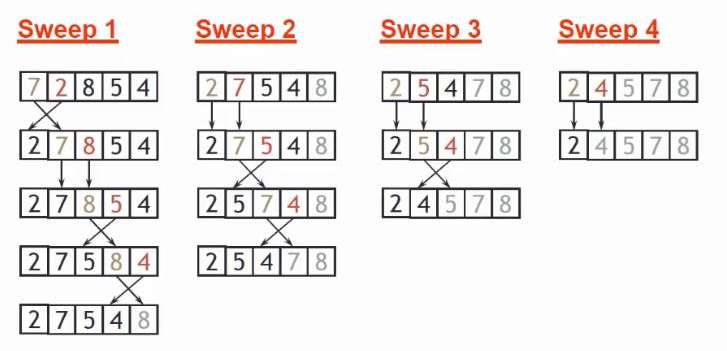
\includegraphics[width=\textwidth]{media/bsort.jpg}
\centering
\end{figure}


Bubble sort runs in $\mathcal{O}(n^2)$ in the best case and the worst case. 

While we are not too concerned about the implementation of algorithms in this class, Bubble Sort is fairly simple to implement, so is it presented below:

\begin{lstlisting}
void bubbleSort(int[] a) {
    int outer, inner;
    
    for (outer = a.length - 1; outer > 0; outer--) {
        for (inner = 0; inner < outer; inner++) {
            if (a[inner] > a[inner + 1]) {
                swap(a, inner, inner + 1);
            }
        }
    }

    void swap(int[] a, int x, int y) {
        int temp = a[x]; a[x] = a[y]; a[y] = temp;
    }

}
\end{lstlisting}

\subsection{Selection Sort}

The selection sort algorithm works by iteratively sweeping through shrinking portions of our list, selecting the smallest element found in each sweep, and swapping the element with the front of the current list. The image below demonstrates how the algorithm works:
 
\begin{figure}[h]
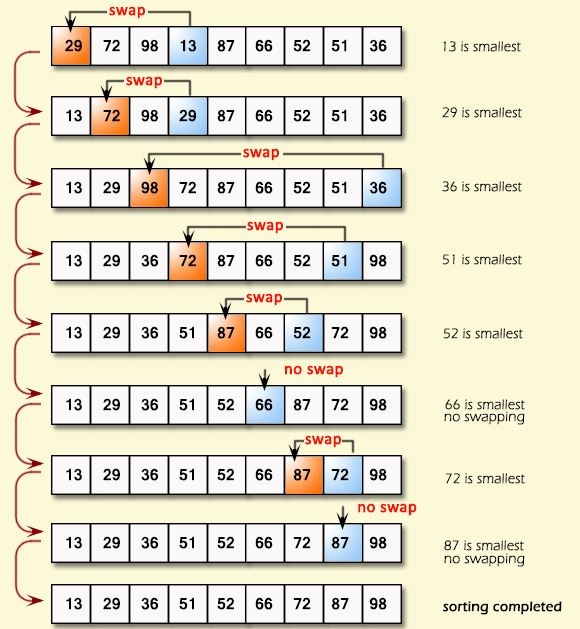
\includegraphics[width=\textwidth, height=15cm]{media/ssort.jpg}
\centering
\end{figure}

\newpage


Like Bubble Sort, Selection Sort also runs in $\mathcal{O}(n^2)$ time in the best case and the worst case. One possible implementation is selection sort is as follows:

\begin{lstlisting}
void selectionSort(int[] a) {
    int outer, inner, min;
    
    for (outer = 0; outer < a.length - 1; outer++) {
        min = outer;
        for (inner = outer + 1; inner < a.length; inner++) {
            if (a[inner] < a[min] {
                min = inner;
            }
        }
        swap(a, outer, min);
    }
}
\end{lstlisting}


\subsection{Insertion Sort}

Insertion sort is very similar to the method that people typically use when they're sorting cards. Although this algorithm runs in $\mathcal{O}(n^2)$ worst case time, it is the preferred algorithm when data is nearly sorted or when the size of the data to sort is small (due to the low overhead). This algorithm has a simple implementation, and it's more efficient in practice than most simple quadratic sorting algorithms. 

Insertion sort works by iteratively grows a sorted output list by removing one element from the data, finding its correct location, and placing it there. This happens until no input elements remain. 

Once again, we are not too concerned with implemenetation details. This is a good illustration of how insertion sort works:  \url{https://upload.wikimedia.org/wikipedia/commons/9/9c/Insertion-sort-example.gif}.

Insertion sort's best case runtime is $\mathcal{O}(n)$. One instance in which this best case behavior is exhibited is when the input list is already sorted. Moreover, since insertion sort performs better on already-sorted lists, we can conclude that insertion sort is an adaptive algorithm as well.


\subsection{Tree Sort}

The tree sort algorithm is fairly simple from a high-level perspective. We insert all of the elements into a binary search tree, and we perform an in-order traversal on the tree. The order in which we process the nodes is also the order that the nodes should be in the final output array. This algorithm runs in $\mathcal{O}(n\log(n))$ time in the average and worst case, and it runs in $\mathcal{O}(n)$ time in the worst case (when we make a degenerate tree).

\subsection{Mergesort}

Mergesort is more complicated than the sorting algorithms we've seen so far. The general approach to performing mergesort is as follows:

\begin{enumerate}
    \item Partition the list of elements into two lists (the two lists should be equally-sized or off by one).
    \item Recursively sort both lists. 
    \item Given the two sorted lists, merge them both into one sorted list. This is done by iteratively examining the head of both lists, and moving the smaller to the end of the new list. 
\end{enumerate}

The runtime of this algorithm is $\mathcal{O}(n\log(n))$ in the average case and the worst case. When we use Java's \verb!Collections.sort!, Mergesort is the algorithm that's used. This algorithm can be implemented externally or internally, and it uses additional memory to perform the merging step (so the algorithm is NOT in-place). Mergesort is stable. 

The heart of the MergeSort algorithm is demonstrated through this code:

\begin{lstlisting}
/* x denotes the lower end of the array region to be sorted, and y denotes the upper end of the array region to be sorted. */
void mergeSort(int[] a, int x, int y) {
    int mid = (x + y)/2;
    if (x != y) {
        mergeSort(a, x, mid);
        mergeSort(a, mid + 1, y);
        merge(a, x, y, mid);
    }
}

void merge(int[] a, int x, int y, int mid) {
    /* This function merges two adjacent sorted lists in an array. Implementation not shown. */
}
\end{lstlisting}